% -*- latex -*-
%%%%%%%%%%%%%%%%%%%%%%%%%%%%%%%%%%%%%%%%%%%%%%%%%%%%%%%%%%%%%%%%
%%%%%%%%%%%%%%%%%%%%%%%%%%%%%%%%%%%%%%%%%%%%%%%%%%%%%%%%%%%%%%%%
%%%%
%%%% This text file is part of the source of 
%%%% `Parallel Programming in MPI and OpenMP'
%%%% by Victor Eijkhout, copyright 2012-6
%%%%
%%%% mpi-functional.tex : about functional parallelism
%%%%
%%%%%%%%%%%%%%%%%%%%%%%%%%%%%%%%%%%%%%%%%%%%%%%%%%%%%%%%%%%%%%%%
%%%%%%%%%%%%%%%%%%%%%%%%%%%%%%%%%%%%%%%%%%%%%%%%%%%%%%%%%%%%%%%%

%\input chapters/mpi-idiom-func
\Level 0 {The SPMD model}

MPI programs conform\footnote{Usually, but not necessarily.}
to the \acf{SPMD} model, where each processor runs the same executable.
This running executable we call a \indexterm{process}.

When MPI was first written, 20 years ago, it was clear what a processor
was: it was what was in a computer on someone's desk, or in a rack.
If this computer was part of a networked cluster, you called it a \indexterm{node}.
So if you ran an MPI program, each node would have one MPI process;
%
\begin{figure}[ht]
  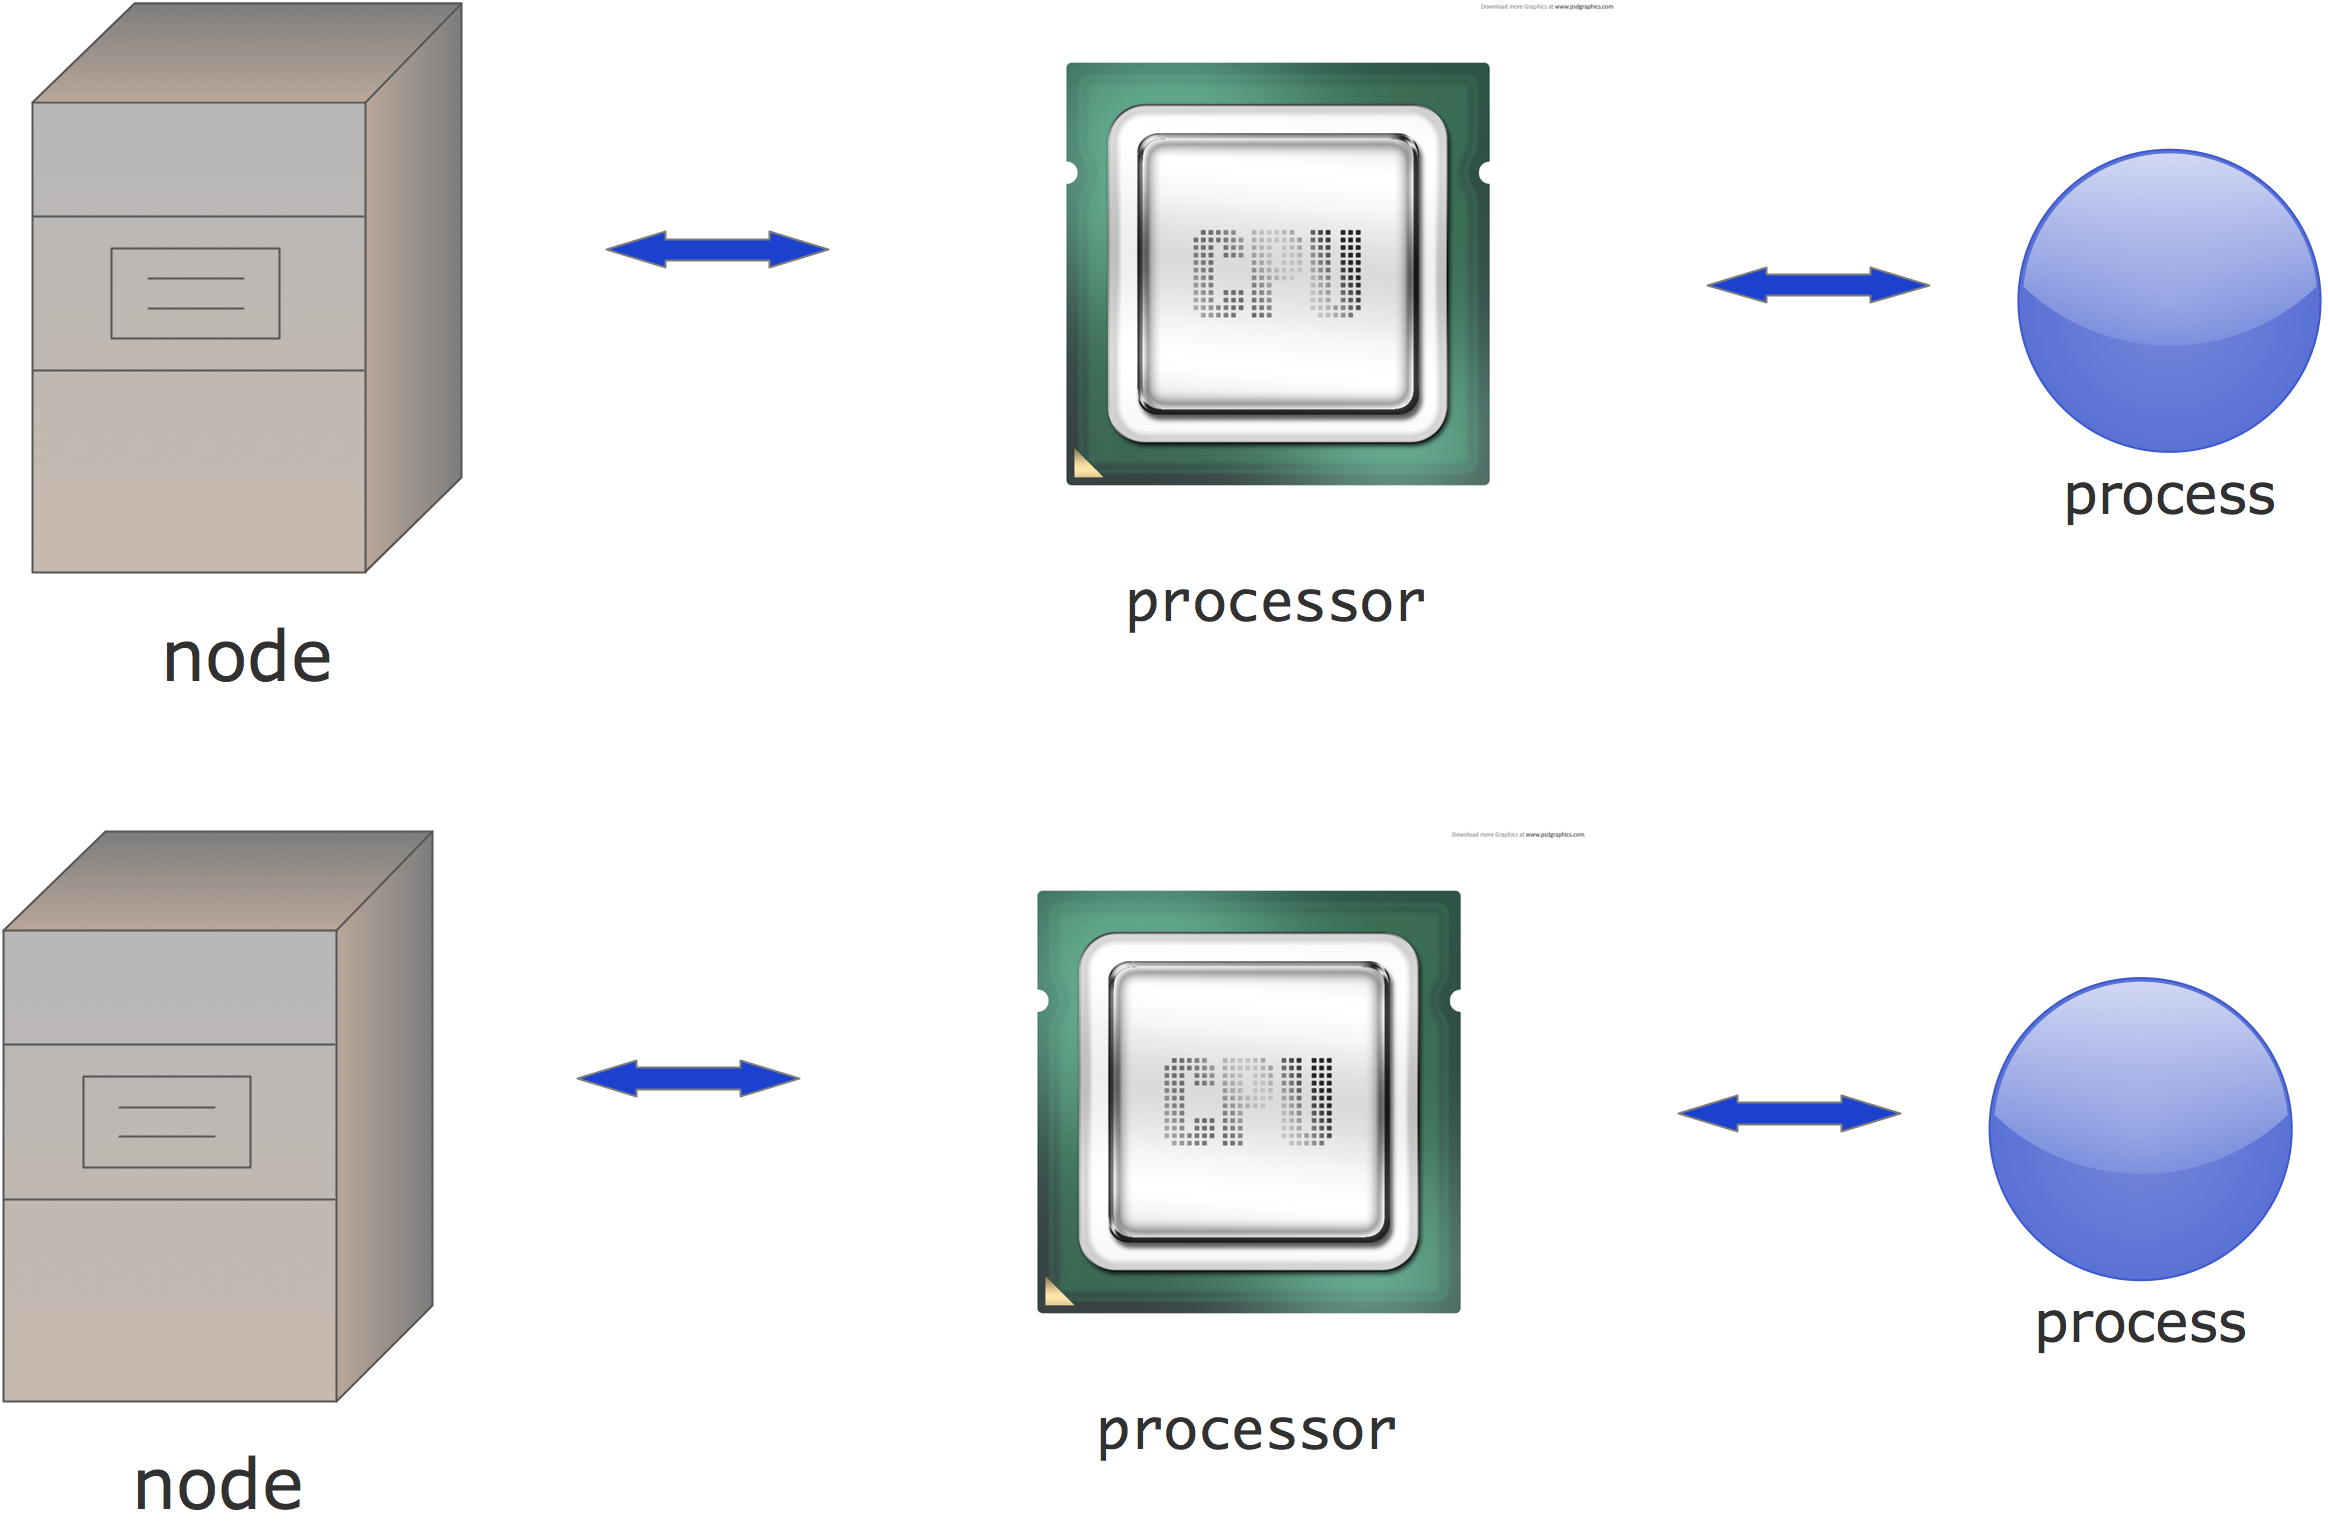
\includegraphics[scale=.11]{mpi-node1}
  \caption{Cluster structure as of the mid 1990s}
  \label{fig:oldmpi}
\end{figure}
%
figure~\ref{fig:oldmpi}.

These days the situation is more complicated.
You can still talk about a node in a cluster, but now a node can contain
more than one processor chip (sometimes called a \indextermdef{socket}),
and each processor chip probably has multiple
\emph{cores}\index{core}.
%
\begin{figure}[ht]
  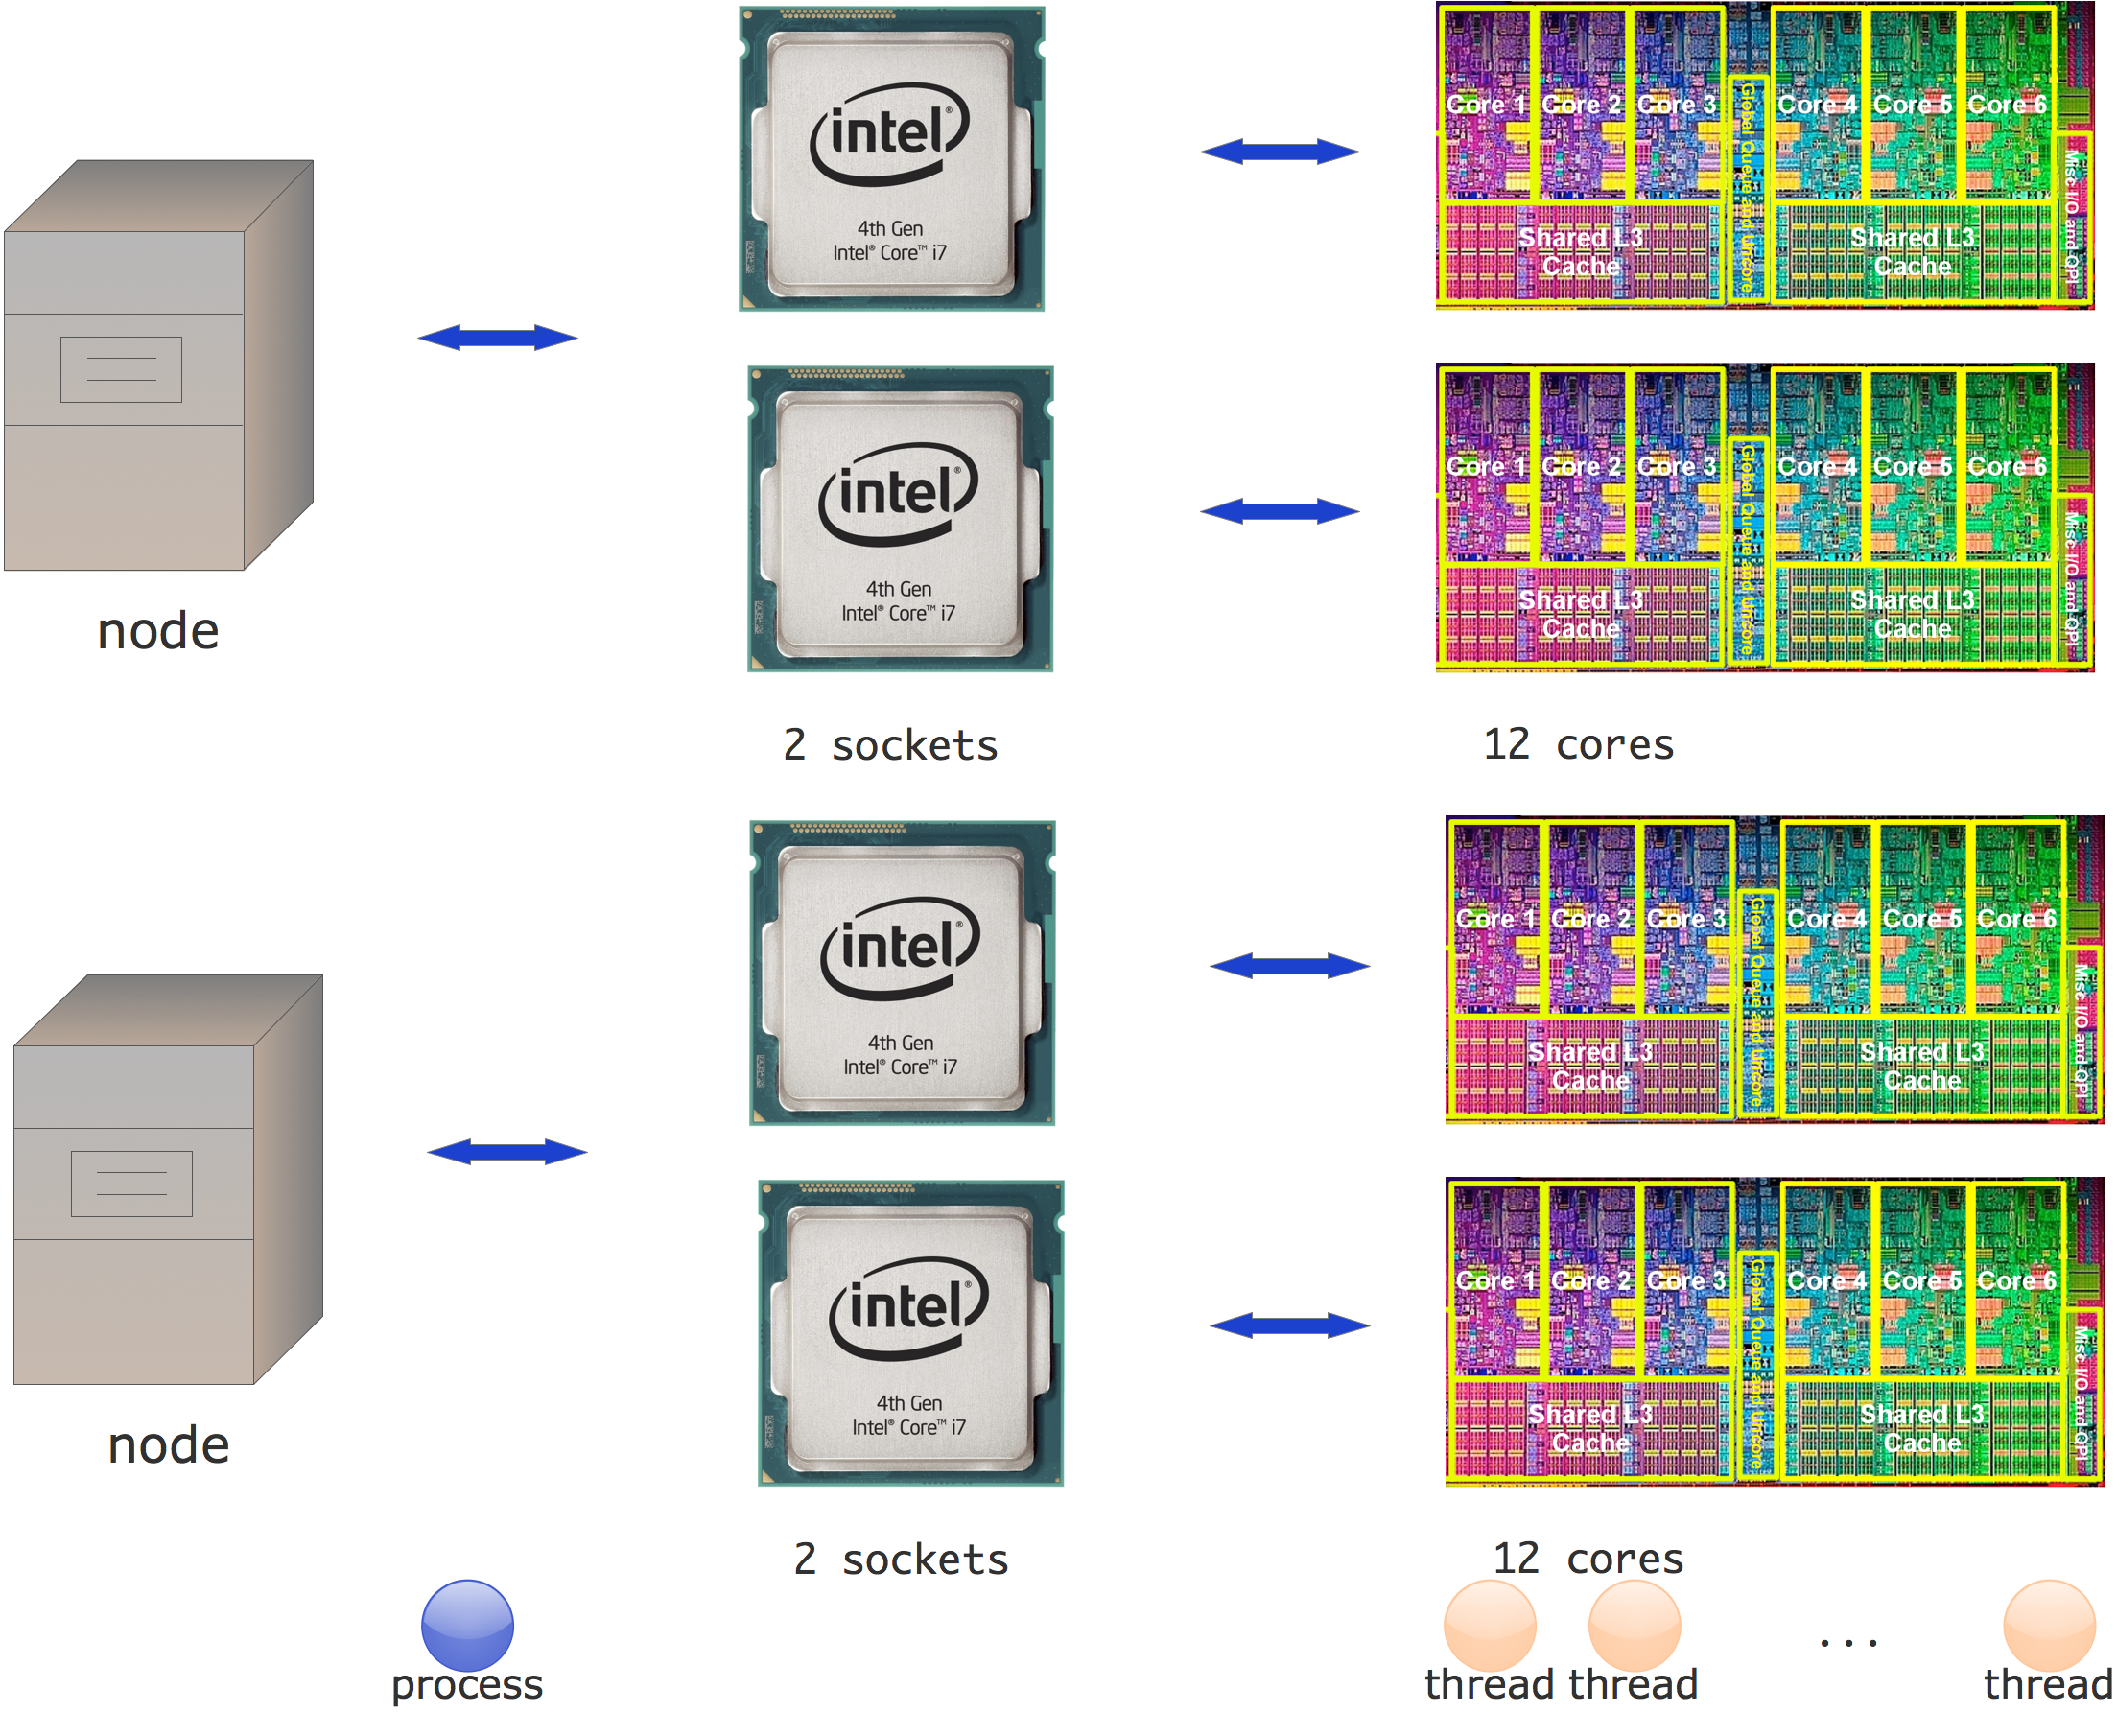
\includegraphics[scale=.11]{mpi-node3}
  \caption{Hybrid cluster structure}
  \label{fig:hybridmpi}
\end{figure}
%
Figure~\ref{fig:hybridmpi} shows how you could explore this using a mix
of MPI between the nodes, and a shared memory programming system on the nodes.

However, since each core can act like an independent processor,
you can also have multiple MPI processes per node. To MPI the cores look
like the old completely separate processors. This is the `pure MPI'
model of figure~\ref{fig:purempi} which we will use in most of this part
of the book.
%
\begin{figure}[ht]
  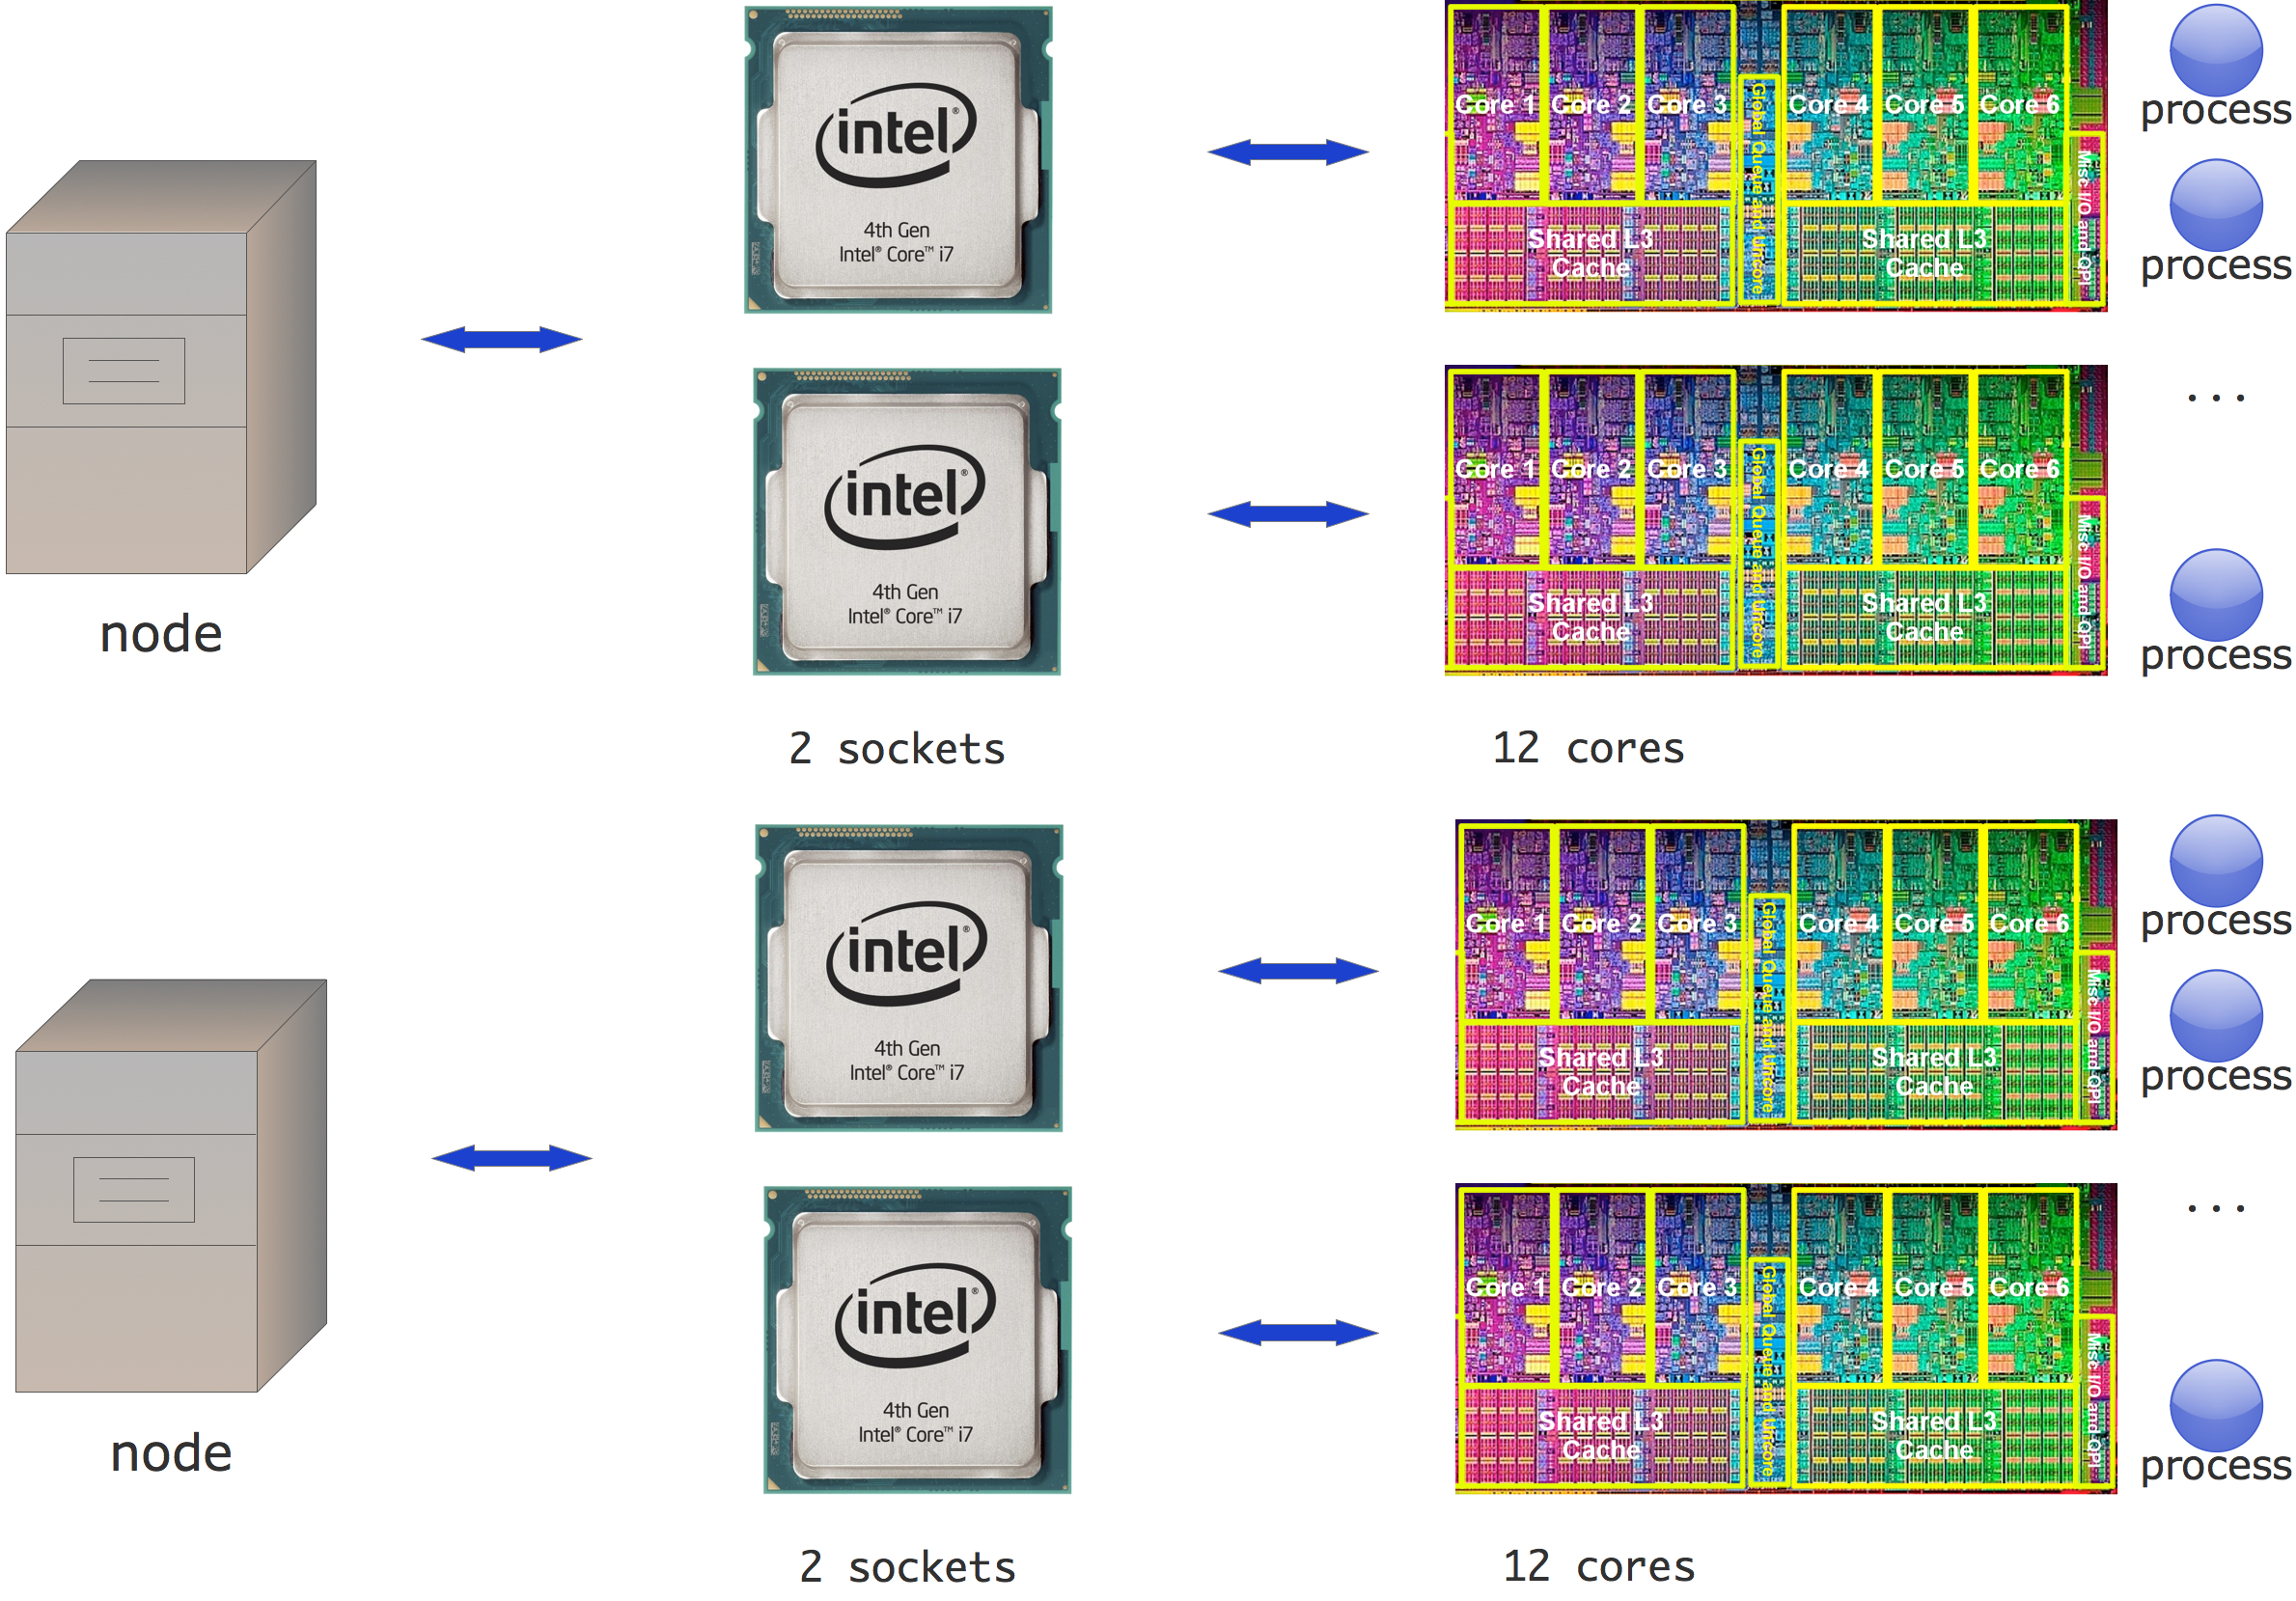
\includegraphics[scale=.11]{mpi-node2}
  \caption{MPI-only cluster structure}
  \label{fig:purempi}
\end{figure}
%

This is somewhat confusing: the old processors needed MPI programming, because
they were physically separated. The cores on a modern processor, on the other hand,
share the same memory, and even some caches. In its basic mode MPI
seems to ignore all
of this: each core receives an MPI process and the programmer writes the same send/receive call no matter
where the other process is located. In fact, you can't immediately see
whether two cores are on the same node or different nodes. (Of course,
on the implementation level MPI uses a different communication
mechanism depending on whether  cores are on the same socket, or on
different nodes.)

%% \Level 0 {Starting and running MPI processes}
\input chapters/mpi-running

%% \Level 0 {Processor identification}
\input chapters/mpi-rank

\Level 0 {Functional parallelism}

Being able to tell processes apart is already enough for some
applications.  Based on its rank, a processor can find its section of
a search space.  For instance, in \indexterm{Monte Carlo codes} a
large number of random samples is generated and some computation
performed on each. (This particular example requires each MPI process
to run an independent random number generator, which is not entirely
trivial.)

\begin{exercise}
  \label{ex:primetest}
  Is the number $N=2,000,000,111$ prime?  Let each process test a
  range of integers, and print out any factor they find.  You don't
  have to test all integers~$<N$: any factor is at
  most~$\sqrt N\approx 45,200$.

  (Hint: \verb+i%0+ probably gives a runtime error.)
\end{exercise}

As another example, in \indexterm{Boolean satisfiability} problems
a number of points in a search space needs to be evaluated. Knowing
a process's rank is enough to let it generate its own portion of the
search space. The computation of the \indexterm{Mandelbrot set} can
also be considered as a case of functional parallelism. However, the
image that is constructed is data that needs to be kept on one
processor, which breaks the symmetry of the decomposition.

Of course, at the end of a functionally parallel run you need to
summarize the results, for instance printing out some total.
The mechanisms for that you will learn next.

%\input chapters/mpi-intro-func

